

Numerical transport calculations have a huge advantage over the analytical
calculation: once a formalism is implemented, it works for arbitrary
configurations within the limits of the model. However it doesn't generally
supply us with data that enhances physical understanding, so its best use as a
means to expand on analytical calculations which we already understand.

In that spirit we performed numeric calculations, simulating a sample with
Rashba Spin-orbit coupling, and spin-resolved leads attached at the edges.

The calculation follows this rough scheme:

\begin{itemize}
    \item Set up the Hamiltonian $H$
    \item Calculate the self-energy matrices $\Sigma_p$
    \item Calculate the Green's functions $G^A$ and $G^R$ by inverting
          $H + \sum_p \Sigma_p$
    \item Use the Fisher-Lee relation to calculate the transmission matrix $T$
            from $G^R$, $G^A$ and $\Sigma_p$
\end{itemize}

\section*{Performance consideration}

These numeric calculations are computationally expensive. If we simulate a
lattice with a total of $n \x n$ sites, the matrices $H$, $\Sigma_p$, $G^R$ and
$G^A$ are of dimensions $2n^2 \times 2n^2$. Inversion of an $m \times m $
matrix and multiplication of two $ m \times m $ matrices both take $O(m^3)$
steps\footnote{There are matrix product algorithms with slightly better
asymptotic scaling, but they are usually very complicated, numerically badly
conditioned, or only advantageous for huge systems; usually all three apply}
\cite{matrixperformance}. All other steps are faster, and can be ignored for
an asymptotic analysis.

So the naive approach takes $O(n^6)$ steps for $n$ lattice sites.

An alternative approach, the \emph{Recursive Green's Function method} works by
decomposing the sample into slices in such a way that the sites in each slice
only interact with neighbor slices. For short range interactions such a
decomposition can be found, and for nearest-neighbor hopping the time
complexity approaches $O(n^3)$ \cite{rgfschmelcher}. However this is payed by
a significantly increased implementation complexity, and the algorithm is tied
to the specific form of the Hamiltonian.

\begin{figure}
    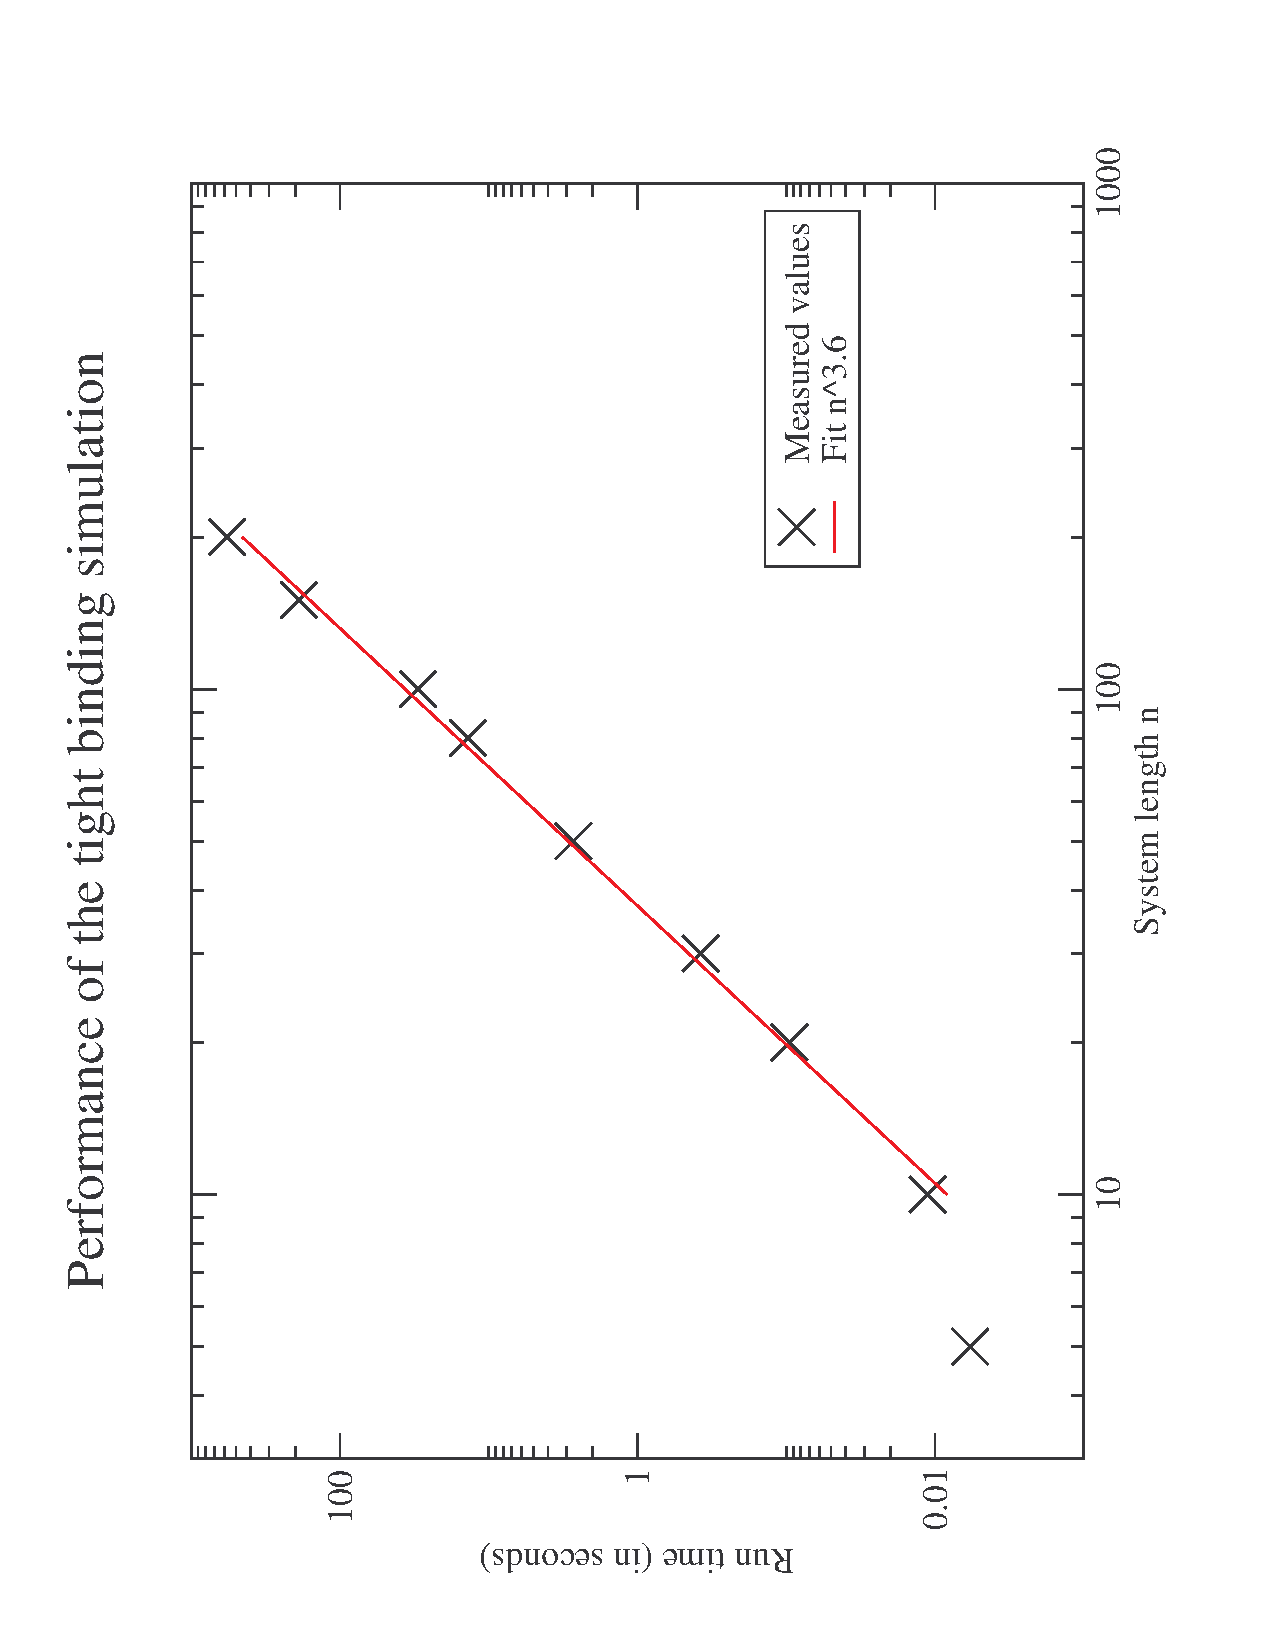
\includegraphics[angle=270,width=0.7\textwidth]{scaling.pdf}
    \caption{Scaling of run time with system size for the tight binding
        simulation, implemented with sparse matrices and the SuperLU sparse
        direct solver. The data was recorded for square samples including
        Rashba spin-orbit coupling, and 4 leads of the same width as the
        sample, on a 2.9GHz AMD64 computer with SSE and 8GB RAM.
        The run time approximately scales as $t(n) = 2
        n^{3.64}\mu s$}
        \label{fig:scaling}
\end{figure}

We chose a middle ground: the "naive" approach, but implemented with sparse
matrices, and using an efficient sparse direct solver\cite{superlu99} for
computing the Green's functions.

The run time thus depends largely on the number of non-zeros in the $H$ and
$\Sigma_p$, and thus on the nature of the interaction. For nearest neighbor
hopping and Rashba spin-orbit coupling we observed a run time scaling of
$O(n^{3.64})$ (See Fig. \ref{fig:scaling}).

\section*{Numerical stability}

The numerical
calculation uses floating point numbers with limited machine precision,
therefore numerical errors are inevitable.

The transmission matrix for a sample which is connected to multiple uniform
leads (with same number of modes per lead) has to fulfill the sum rules

\begin{align}
    \sum_p T_{pq} = \sum_q T_{pq} = M
\end{align}

Where $M$ is the number of modes (and thusly and integer). We can calculate
this left hand side of this equation from the numerical simulation, round it
to the nearest integer and thus estimate the numerical error in $T_{pq}$.

Since generally matrix inversion is numerically worse conditioned than solving
a linear equation system\cite{matrixinversion}, we don't actually compute
$G^A$ and $G^R$, but rather the products $G^A\Sigma_p$ and $G^R\Sigma_q$,
which can be written as solutions of linear equation systems.

\begin{align}
    X_p &= \Sigma_p G^R\\
    X_p^\dagger &= (G^R)^\dagger \Sigma_p^\dagger = G^A \sigma_p^\dagger\\
    \Rightarrow\quad (G^A)^-1 X_p^\dagger &= \Sigma_p^\dagger
    \label{eq:lin_gls}
\end{align}

Eq. \ref{eq:lin_gls} is the form with which linear sparse solvers typically
work. They typically calculate a LU decomposition (that is they write
$(G^A)^-1 = L \cdot U$, where $L$ is a lower triangular matrix and $U$ an
upper triangular matrix), and directly solve the equation by elimination.
Complex conjugation and transposition of $X_p^\dagger$ finally gives us the
matrix which we need evaluating the Fischer-Lee relation.

% vim: ts=4 sw=4 expandtab spell spelllang=en_us tw=78
